%\documentclass[handout]{beamer}
\documentclass{beamer}

%-----------------------------
%           PACKAGES

\usepackage[T1]{fontenc}
\usepackage[utf8]{inputenc}
\usepackage{eulervm}
\usepackage[scaled]{helvet}
\usepackage{graphicx}
\usepackage{amsmath,amsfonts,amssymb}
\usepackage{tikz}
\usepackage{multicol}
\usepackage{array,multirow,makecell}
\usepackage{color}
\usepackage{transparent}


\usetheme{Warsaw}
%\usetheme{Antibes}
%\usetheme{Montpellier}
%\usetheme{JuanLesPins}
%\usetheme{Goettingen}
\usefonttheme[onlymath]{serif}
\usecolortheme{Ben}
%\usecolortheme{fly}


\newcolumntype{K}[1]{>{\centering\arraybackslash}p{#1}}

\makeatletter
\def\insertsectionnavigation#1{%
  \hbox to #1{\vbox{{\usebeamerfont{section in head/foot}%
     \usebeamercolor[fg]{section in head/foot}%
     \def\slideentry##1##2##3##4##5##6{}%
     \def\sectionentry##1##2##3##4##5{%
       \ifnum##5=\c@part%
       \def\insertsectionhead{##2\hskip1em}%
       \def\insertsectionheadnumber{##1}%
       \def\insertpartheadnumber{##5}%
         \hyperlink{Navigation##3}{%
             \ifnum\c@section=##1%
               {\usebeamertemplate{section in head/foot}}%
             \else%
               {\usebeamertemplate{section in head/foot shaded}}%
             \fi%
         }\par
       \fi}%
       \parbox[c][0cm][c]{.5\paperwidth}{%
       \begin{multicols}{2}
       \dohead
       \end{multicols}}\space}
     }%
  \hfil}%
}

\def\insertsubsectionnavigation#1{%
  \hbox to #1{%
    \vbox{{%
      \usebeamerfont{subsection in head/foot}\usebeamercolor[fg]{subsection in head/foot}%
      \vskip0.5625ex%
      \beamer@currentsubsection=0%
      \def\sectionentry##1##2##3##4##5{}%
      \def\slideentry##1##2##3##4##5##6{\ifnum##6=\c@part\ifnum##1=\c@section%
        \ifnum##2>\beamer@currentsubsection%
        \beamer@currentsubsection=##2%
        \def\insertsubsectionhead{##5}%
        \def\insertsectionheadnumber{##1}%
        \def\insertsubsectionheadnumber{##2}%
        \def\insertpartheadnumber{##6}%
        \beamer@link(##4){%
              \ifnum\c@subsection=##2%
                {\usebeamertemplate{subsection in head/foot}}%
              \else%
                {\usebeamertemplate{subsection in head/foot shaded}}%
              \fi\hfill}\par
        \fi\fi\fi}%
       \hspace*{0.5em}\parbox[c][0cm][c]{\dimexpr.5\paperwidth-1em\relax}{%
       \begin{multicols}{2}
       \dohead\vskip0.5625ex\end{multicols}
       }\space
   }\hfil
}}}

\setbeamertemplate{headline}
{%
  \leavevmode\@tempdimb=2.4375ex%
  \ifnum\beamer@subsectionmax<\beamer@sectionmax%
    \multiply\@tempdimb by\beamer@sectionmax%
  \else%
    \multiply\@tempdimb by\beamer@subsectionmax%
  \fi%
  \ifdim\@tempdimb>0pt%
    \advance\@tempdimb by 1.125ex%
    \begin{beamercolorbox}[wd=.5\paperwidth,ht=0.5\@tempdimb,dp=2ex]{section in head/foot}%
      \vbox to0.5\@tempdimb{\vfill\insertsectionnavigation{.5\paperwidth}\vfill}%
    \end{beamercolorbox}%
    \begin{beamercolorbox}[wd=.5\paperwidth,ht=0.5\@tempdimb,dp=2ex]{subsection in head/foot}%
      \vbox to0.5\@tempdimb{\vfill\insertsubsectionnavigation{.5\paperwidth}\vfill}%
    \end{beamercolorbox}%
  \fi%
}
\makeatother

\usetikzlibrary{positioning,arrows}
\usetikzlibrary{decorations.pathmorphing}
\usetikzlibrary{decorations.markings}



\newcommand{\grille}{
    \begin{tikzpicture}[overlay,remember picture]
        \begin{scope}[shift={(current page.south west)}]
            \draw[gray!50] (0,0) grid[step=2mm] (current page.north east);
            \draw[red!50] (0,0) grid[step=1cm] (current page.north east);
            \draw (0.2,1) node {1};
            \draw (0.2,2) node {2};
            \draw (0.2,3) node {3};
            \draw (0.2,4) node {4};
            \draw (0.2,5) node {5};
            \draw (0.2,6) node {6};
            \draw (0.2,7) node {7};
            \draw (0.2,8) node {8};
            \draw (0.2,9) node {9};
            \draw (1,0.5) node {1};
            \draw (2,0.5) node {2};
            \draw (3,0.5) node {3};
            \draw (4,0.5) node {4};
            \draw (5,0.5) node {5};
            \draw (6,0.5) node {6};
            \draw (7,0.5) node {7};
            \draw (8,0.5) node {8};
            \draw (9,0.5) node {9};
            \draw (10,0.5) node {10};
            \draw (11,0.5) node {11};
            \draw (12,0.5) node {12};
        \end{scope}
    \end{tikzpicture}
}
\newcommand{\degres}{\ensuremath{^\circ}}
\title[Ph. D. defense]{Développement d'une échelle double face pour la trajectométrie en physique des hautes énergies.}
\subtitle{Ph. D. defense}
\institute{DESY}
\author[Benjamin BOITRELLE]{Benjamin BOITRELLE  \\ Supervisors: Jérôme Baudot, Ingrid Maria Gregor} %\\ On behalf of the PLUME Collaboration
\date{February 13, 2017}
\defbeamertemplate*{footline}{shadow theme}
%\titlegraphic{\includegraphics[scale = 0.08]{Pictures/DESY-Logo.png}}
{%
    \leavevmode%
    \hbox{\begin{beamercolorbox}[wd=.5\paperwidth,ht=2.5ex,dp=1.125ex,leftskip=.3cm plus1fil,rightskip=.3cm]{author in head/foot}%
            \usebeamerfont{author in head/foot}\insertframenumber\,/\,\inserttotalframenumber\hfill\insertshortauthor
        \end{beamercolorbox}%
        \begin{beamercolorbox}[wd=.5\paperwidth,ht=2.5ex,dp=1.125ex,leftskip=.3cm,rightskip=.3cm plus1fil]{title in head/foot}%
            \usebeamerfont{title in head/foot}\insertshorttitle%
    \end{beamercolorbox}}%
    \vskip0pt%
}

%-------------
%
% INTRODUCTION:
%   - What is the SM?
%   - Higgs boson
%   - ILC and ILD
%
% WORK:
%   - PLUME and CMOS
%   - Impact parameter
% 
% CONCLUSION AND OUTLOOK

\begin{document}

  \begin{frame}[plain]
    \maketitle
    \begin{columns}[t]
        \begin{column}{2cm}
            \includegraphics[width = 2cm, height = 2cm]{Pictures/DESY-Logo.png}
        \end{column}

        \begin{column}{3cm}
            \includegraphics[width = 3cm, height = 2cm]{Pictures/logo_IPHC_10cm.png}
        \end{column}
        \begin{column}{3cm}
            \includegraphics[width = 3cm, height = 2cm]{Pictures/logo_uni_stra.jpg}
        \end{column}        
        \begin{column}{3cm}
            \includegraphics[width = 3cm, height = 1.5cm]{Pictures/logo_plume.png}
        \end{column}
    \end{columns}

  \end{frame}

  \begin{frame}[plain]
    \frametitle{Outlines}

    \tableofcontents
  \end{frame}

  \section{Introduction}
    \subsection{Standard Model}

    \begin{frame}
      %\frametitle{Standard Model}
      \frametitle{What is the Universe made of?}

      \begin{block}{Matter:}
      \begin{center}
        \begin{tabular}{c c c c c c c}
        \multirow{3}*{\uncover<1->{Fermions}} & \multicolumn{3}{ c }{\uncover<2->{Leptons}} & \multicolumn{3}{ c }{\uncover<2->{Quarks}} \tabularnewline
          & \uncover<3->{$e^-$ & $\mu$ & $\tau$} & \uncover<4->{$u$ & $c$ & $t$} \tabularnewline 
          & \uncover<3->{$\nu_{e}$ & $\nu_{\mu}$ & $\nu_{\tau}$} & \uncover<4->{$d$ & $s$ & $b$ } \tabularnewline 
          
        \end{tabular}
        %\includegraphics[width = 0.6\textwidth]{Pictures/elementaryParticles.jpg}
      \end{center}
      \end{block}
      \uncover<5->{\begin{block}{Forces:}
      \begin{center}
        \begin{tabular}{c c c c}
        \multirow{5}*{\uncover<5->{Bosons}} & \uncover<6->{$\gamma$} & \uncover<6->{$\rightarrow$} & \uncover<6->{E.M. interaction} \tabularnewline
        & \uncover<7->{$Z^{0}/W^{\pm}$} & \uncover<7->{$\rightarrow$} & \uncover<7->{Weak interaction} \tabularnewline
        & \uncover<8->{$g$ & $\rightarrow$} & \uncover<8->{Strong interaction} \tabularnewline
        & \uncover<9->{\textcolor{gray}{graviton} & \textcolor{gray}{$\rightarrow$}} & \uncover<9->{\textcolor{gray}{Gravitation}} \tabularnewline
        %\only<11->{\hline}
        & \uncover<10->{$H$ & $\rightarrow$} & \uncover<10->{Higgs field} \tabularnewline
        \end{tabular}
      \end{center}
      \end{block}}

    \end{frame}

    \begin{frame}
      \frametitle{Open questions}

      \begin{alertblock}{Limitations}
        \begin{itemize}
          \item Free parameters
          \item Neutrino mass
          \item Dark matter and dark energy
          \item ...
        \end{itemize}
      \end{alertblock}
      
      \begin{block}{Other theories}
        \begin{itemize}
          \item SUSY
          \item GUT
          \item Technicolor
          \item ...
        \end{itemize}
      \end{block}
    \end{frame}

    \subsection{Higgs Boson}

    \begin{frame}
      \frametitle{The Higgs boson discovery}

      \begin{columns}[t]
        \begin{column}{5cm}
          \begin{itemize}
            \item Discovery at the LHC (ATLAS and CMS)
          \end{itemize}
        \end{column}
        \begin{column}{5cm}
        elele
        \end{column}
      \end{columns}
    \end{frame}

    \begin{frame}
      \frametitle{Higgs Boson}

      \begin{center}
        \includegraphics[width = 0.6\textwidth]{Pictures/Chapter_Theory_figs_mass-coupling1TeV.png}
      \end{center}
     
    \end{frame}
    \subsection{ILC and ILD}
%-------------------------------
%   Intro: ILC 
%-------------------------------

  \begin{frame}
    \frametitle{International Linear Collider}

    \vspace{-0.3cm}
    \begin{center}
      \includegraphics[width = 9 cm]{Pictures/ILC.png}
    \end{center}

    \vspace{-0.3cm}
    \begin{itemize}
      \item Future $\rm{e}^+\rm{e}^-$ linear collider at $\sqrt{s} = 250 - 500~\rm{GeV}$ \\ (upgrade up to $\sqrt{s} = 1~\rm{TeV}$)
      \item Polarised beam
      \item Luminosity $\simeq 2 \times 10^{34}~\rm{cm}^{-2}\rm{s}^{-1}$
      \item Candidate site: Kitakami in nothern Japan
      \item To study properties of the Higgs boson, top physics...
    \end{itemize}
  \end{frame}
 
 %-------------------------------
%                           Intro: ILD VS SiD 
%-------------------------------

\begin{frame}
  \frametitle{SiD and ILD}

  \vspace{-0.12cm}
  \begin{columns}[t]
    \begin{column}{5cm}
      \includegraphics[width = 5cm, height = 2.9 cm]{Pictures/ILC_SiD.jpg}
      \vspace{-0.25cm}
      \begin{block}{Silicon Detector}
        \footnotesize{
        \begin{itemize}
          \item Silicon tracking \\ (radius = 1.2m)
          \item B$_{field}$ = 5 T
        \end{itemize}
        }
      \end{block}
    \end{column}

    \begin{column}{5cm}
      \includegraphics[width = 5cm, height = 2.9 cm]{Pictures/ILD_all_110826.jpg}
      \vspace{-0.25cm}
      \begin{block}{International Linear Detector}
        \footnotesize{
        \begin{itemize}
          \item TPC + silicon envelope \\ (radius = 1.8 m)
          \item B$_{field}$ = 3.5 T
        \end{itemize}
        }
      \end{block}
    \end{column}
  \end{columns}

  \vspace{-0.2cm}
  \begin{block}{Both detectors designed for Particle Flow Calorimetry}
    \footnotesize{
    \begin{itemize}
      \item High granularity calorimeters (ECAL and HCAL) inside solenoid
        \vspace{-0.1cm}
      \item Low mass tracker to reduce interactions and conversions
    \end{itemize}
    }
  \end{block}
  
\end{frame}
  
\begin{frame}
    \frametitle{Overview of the ILD}

    \begin{center}
        \includegraphics[width = 11cm]{Pictures/ild-detector-ilc.jpg}
    \end{center}
\end{frame}

  
  \begin{frame}[label=vxd]
    \frametitle{The ILD Vertex Detector}

    \vspace{-0.3cm}
    \begin{block}{Two geometry options}
      \begin{center}
        \includegraphics[width = 6 cm,height = 2.8cm]{Pictures/ild_VXD.png}
      \end{center}
      \vspace{-0.5cm}
      \begin{columns}[t]
        \begin{column}{5cm}
          5 single-sided layers
        \end{column}
        \begin{column}{5cm}
          3 double-sided layers
        \end{column}
      \end{columns}
    \end{block}

    \vspace{-0.2cm}
    \begin{alertblock}{Impact parameter resolution}
        \begin{itemize}
            \item $\sigma_{r\phi} \simeq \sigma_{rz} \simeq a \oplus \frac{b}{p \cdot sin^{3/2} \theta}$
            \item Hit resolution: $a \simeq 5 \mu m \Rightarrow ~ \sigma_{spatial} < 3 \mu m$
            \item Multiple scattering: $b \simeq 10 - 15 \mu m \Rightarrow$ material budget per layer $\simeq 0.15~\%$ X$_0$ 
        \end{itemize}

    \end{alertblock}

    %\vspace{-0.25cm}
    %\begin{alertblock}{The ILC vertex detector requirements}
    %    \begin{itemize}
    %        %\item $\sigma_{r\phi} \simeq \sigma_{rz} \simeq a \oplus \frac{b}{p \cdot sin^{3/2} \theta}$
    %        %\item Hit resolution: $a \simeq 5 \mu m \Rightarrow \ \sigma_{spatial} < 3 \mu m$
    %        %\item Multiple scattering: $b \simeq 10 - 15 \mu m \Rightarrow$ material budget per layer $\simeq 0.15 \% \ X_0 $ for an excellent flavour tagging performance. 
    %        \item Spatial resolution: $< \ 3~\mu m$
    %        \item Material budget per measurement point: $\simeq 0.15~\%~X_0 $
    %    \end{itemize}
    %\end{alertblock}

    %\vspace{-0.24cm}
    %\begin{center}
    %    \includegraphics[width = 6 cm,height = 2.8cm]{Pictures/ild_VXD.png}

    %    %\vspace{-0.2cm}
    %    \scriptsize{Two geometry options for the ILD vertex detector: 5 layers of single-sided detector (left) or \\ \only<2>{\textbf{3 layers of double-sided detector}} \only<-1>{3 layers of double-sided detector} (right)}

    %\end{center}

\end{frame}

%-------------------------------
%                           PLUME Project
%-------------------------------

  %\section{Vertex detector}
  %  \subsection{CMOS sensors}
  %  \subsection{PLUME project}
  %  \subsection{Impact parameter}
    
\section{PLUME project}
\begin{frame}
    \frametitle{Outlines}
    \tableofcontents[currentsection,hideothersubsections, 
    sectionstyle=show/shaded,]
\end{frame}

%--------------------------------
%       PART I: PLUME

\begin{frame}
  \frametitle{Double-sided VXD: PLUME}

  \begin{columns}[c]
    \begin{column}{3cm}
      \includegraphics[width = 3cm]{Pictures/logo_plume.png}
    \end{column}
    \vspace{-0.2cm}
    \begin{column}{7cm}
      PLUME = \textbf{P}ixelated \textbf{L}adder with \textbf{U}ltra-low \textbf{M}aterial \textbf{E}mbedding
    \end{column}
  \end{columns}

  \begin{columns}[t]
    \begin{column}{1cm}
      \includegraphics[width = 1.5cm]{Pictures/logo_IPHC_10cm.png}
    \end{column}
    \begin{column}{1cm}
      \includegraphics[width = 1cm]{Pictures/DESY-Logo.png}
    \end{column}
    \begin{column}{1cm}
      \includegraphics[width = 2cm]{Pictures/logo_uni_bristol.jpg}
    \end{column}
  \end{columns}

  \vspace{-0.15cm}
  %\begin{block}{Concepit}
  %    \begin{itemize}
  %        \item Double-sided ladder with an active area of 1x12cm$^2$;
  %        \item On each side: six MIMOSA-26 CMOS sensors thinned to 50 $\mu$m;
  %        \item Kapton-metal flex cable;
  %        \item 2 mm of Silicon carbide foam as mechanical support between two modules and spacer.
  %    \end{itemize}
  %\end{block}

  \begin{block}{Motivation}
    ILD Vertex detector at ILC
  \end{block}

  \vspace{-0.18cm}
  \begin{block}{Design}
    \begin{itemize}
      \item Double-sided ladder with an active area of 1x12cm$^2$
      \item On each side: six MIMOSA-26 CMOS sensors thinned down to $\sim 50~\mu$m on a kapton-metal flex cable
      \item 2 mm of silicon carbide foam as mechanical support and spacer between two modules
    \end{itemize}
  \end{block}
\end{frame}

\subsection{Design}
%-------------------------------
%                           PLUME scheme + picture of a module
%-------------------------------

\begin{frame}
  \frametitle{What does it look like?}

  \begin{center}
    \includegraphics[width = 10 cm]{Pictures/PLUME_copper_module.png}

    Picture of one module with copper traces.
  \end{center}

  \vspace{-0.2cm}
  \begin{center}
    \includegraphics[width = 10 cm]{Pictures/scheme_plume.png}

    Scheme of one PLUME ladder.
  \end{center}
\end{frame}

%-------------------------------
%                           FOAM
%-------------------------------

\begin{frame}
  \frametitle{Foam support structure}

  \vspace{-0.6cm}
  \begin{columns}[t]

    \begin{column}{4cm}
      \begin{center}
        \includegraphics[width = 4cm]{Pictures/foam1.png}
      \end{center}
    \end{column}

    \begin{column}{4cm}
      \begin{center}
        \includegraphics[width = 4cm]{Pictures/foam2.png}
      \end{center}
    \end{column}

    \begin{column}{4cm}
      \vspace{-0.2cm}
      \begin{center}
        \begin{block}{Properties}
          \begin{itemize}
            \item Open-cell foam
            \item Macroscopically uniform
            \item No tensioning needed
            \item Density: 4 to 8~\% \\ (2-3~\% possible)
            \item Low thermal and electrical conductivity \\ (50 W/m/K)
          \end{itemize}
        \end{block}
      \end{center}
    \end{column}

  \end{columns}

\end{frame}

%-------------------------------
%                           Mi26 
%-------------------------------

\begin{frame}
  \frametitle{MIMOSA-26 sensor}

  \vspace{-0.5cm}
  \begin{columns}[c]
    \begin{column}{4cm}
      \begin{center}
        %\vspace{-0.3cm}
        \includegraphics[width = 4.0cm,height=3.6cm]{Pictures/mi26.jpg}
      \end{center}
    \end{column}

    \begin{column}{4cm}
      \begin{center}
        \includegraphics[width = 4.0cm]{Pictures/efficiency_mi26.png}

        % \tiny{From IPHC - Strasbourg}
      \end{center}
      %    \begin{center}
      %        \begin{block}{Well known chips}
      %        Used for EUDET style telescopes since 2009
      %        \end{block}
      %    \end{center}
    \end{column}
    \begin{column}{4cm}
      \begin{center}
        \includegraphics[width = 4.0cm, height=3.6cm]{Pictures/pxlFinal_sideView_smallSize.jpg}
      \end{center}
    \end{column}
  \end{columns}

  \begin{block}{Monolithic Active Pixels Sensor (MAPS)}
    \scriptsize{
    \begin{itemize}
      \item Pitch: $18.4~\mu\text{m}$ (square pixels)
      \item Active area: $10.6 \times 21.2 \text{mm}^2$ (576 rows x 1152 columns)
      \item Integration time: $115.2~\mu\text(s)$ ($200~\text{ns}$ per line)
      \item Binary output with \hyperlink{suze}{Zero suppression}
      \item Well known sensors $\Rightarrow$ used for EUDET telescope
      \item Extended to MIMOSA-28 exploited in STAR-PXL vertex detector @ RHIC-BNL since 2014
    \end{itemize}
   }
  \end{block}

  %\vspace{-0.2cm}
  %\scriptsize{
  %  \begin{itemize}
  %    \item Monolithic Active Pixels Sensor 
  %    \item Pitch of 18.4 $\mu m$ (square pixels)
  %    \item Active area: 10.6 x 21.2 mm$^2$ (576 rows x 1152 columns)
  %    \item Column-parallel readout: integration time of 115.2 $\mu$s (200 ns per line) for 80 MHz clock
  %    \item \hyperlink{suze}{Zero suppression} (to optimize data bandwith) with binary output
  %    \item Well known sensors $\Rightarrow$ used for EUDET telescope
  %    \item Extended to MIMOSA-28 exploited in STAR-PXL vertex detector @ RHIC-BNL since 2014
  %  \end{itemize}
  %}
  %\grille
\end{frame}

\subsection{Main aims}
%-------------------------------
%                           Aims
%-------------------------------

\begin{frame}
  \frametitle{Main aims}

  \begin{itemize}
    \item Constraint material budget $\Rightarrow$ $< 0.3~\%$ X$_0$
    \item Study how to implement \hyperlink{powerPulsing}{power pulsing} and its impact on a strong magnetic field
    \item Study the advantage of having two measurement points (\hyperlink{miniVec}{mini vectors})
    \item Study impact of the mechanical structure on sensor performance
    %\item Try to reach a material budget of less than 0.3 \% X$_0$ for double-sided ladders
    %\item Use a \hyperlink{powerPulsing}{power pulsing} (200 ms period) in a strong magnetic field with air cooling to decrease the power consumption of the ladder
    %\item Study of the advantage to have two measurement points in the tracking of a particle (\hyperlink{miniVec}{mini vectors}) 
    %\item Study of the alignment and \textbf{the spatial resolution}
  \end{itemize}
\end{frame}

  \section{Mechanical deformation}
  
\begin{frame}
    \frametitle{Outlines}
    \tableofcontents[currentsection,hideothersubsections, 
    sectionstyle=show/shaded]
\end{frame}

%-------------------------------
%   TB
%-------------------------------

  \subsection{Test Beam @ SPS}
  \begin{frame}
    \frametitle{Test beam @ SPS with 120 GeV $\pi^-$ in November 2011}

    \begin{columns}[t]
      \begin{column}{4cm}
        \begin{center}
          \includegraphics[width = 4 cm]{Pictures/plume_testBeam_nov2011.jpg}
        \end{center}
      \end{column}

      \begin{column}{7cm}
        \vspace{-0.8cm}
        \begin{itemize}
          \item Beam test on line H6a @ SPS
          \item Reference plane: 4 Mimosa 26
          \item Validation of the first double-sided ladder equipped with 12 Mi26 sensors
        \end{itemize}

        \vspace{-0.3cm}
        \begin{block}{Ladder performance studies:}
          \begin{itemize}
            \item In threshold (5 and 6 mV)
            \item In position (sensor 1-2, 3-4 and 5-6)
            \item Without and with angle (between $30^{circ}$ and $40^{circ}$)
            \item With two different air flow speeds ($\simeq 3$ to 6 $\text{ms}^{-1}$)
          \end{itemize}
        \end{block}
      \end{column}
    \end{columns}

    \vspace{0.1cm}
    \footnotesize{
    \centering{Jérôme Baudot, Gilles Claus, Loic Cousin, Mathieu Goffe, Rohrry Gold, Joel Goldstein, Ingrid Gregor, Robert Maria.}}
  \end{frame}

  \begin{frame}
    \frametitle{Test beam @ SPS with 120 GeV $\pi^-$ in November 2011}

    %Beam of 120 GeV $\pi -$.

    \vspace{-0.1cm}
    Three configurations studied:

    \vspace{-0.1cm}
    \begin{columns}[t]
      \begin{column}{4cm}
        \begin{center}
          \includegraphics[width = 4cm,height = 3.9cm]{Pictures/tb_cern_11_sketch_normal.pdf}

          \footnotesize{\textbf{Module perpendicular to the beam.}}
        \end{center}
      \end{column}

      \begin{column}{4cm}
        \begin{center}
          \includegraphics[width = 4cm,height = 4.1cm]{Pictures/tb_cern_11_sketch_tilted.pdf}

          \vspace{-0.2cm}
          \footnotesize{\textbf{Module tilted (between 28\degres and 40\degres).}}
        \end{center}
      \end{column}

      \begin{column}{4cm}
        \begin{center}
          \includegraphics[width = 4cm,height = 4.0cm]{Pictures/tb_cern_11_sketch_tilted120mm.pdf}

          \footnotesize{Module tilted ($\simeq$ 60\degres).}
        \end{center}
      \end{column}
    \end{columns}

    \vspace{0.1cm}
    \footnotesize{$\Rightarrow$ Study track-hit residual and the distribution of this residual as a function of the relative position of the beam on the sensor.

    \vspace{0.1cm}
    \centering{\textbf{Analysis performed with TAF (TAPI Analysis Framework). }}}
    %\grille
\end{frame}

\begin{frame}
    \frametitle{Track-hit residual}

    \begin{columns}[t]
      \begin{column}{7cm}
        \begin{center}
          \includegraphics[width = 7cm]{Pictures/residual_explanation.png}
        \end{center}
      \end{column}
      \begin{column}{4cm}
        \scriptsize{
        \begin{block}{Device Under Test (DUT) alignment:}
          \begin{itemize}
            \item Telescope planes defined particle's track
            \item Alignment of DUT in local coordinate system:
              \begin{itemize}
                \scriptsize{
                \item Define a maximal range in which a hit can be associated to a track
                \item Find the best tilt and position to minimise the distance between a hit and its associated track.
                }
              \end{itemize}
          \end{itemize}
        \end{block}
      }
      \end{column}
    \end{columns}
\end{frame}

%-------------------------------
%                           RUN Normal incidence
%-------------------------------
\begin{frame}
  \frametitle{Module perpendicular to the beam}

  \vspace{-0.2cm}
  \centering{Threshold 6 $\sigma$, air flow speed < 5m/s and 1.8M events.}

  \vspace{-0.2cm}
  \begin{center}
    \begin{columns}[t]
      \begin{column}{4cm}
        \centering
        \includegraphics[width = 4cm, height = 1.8cm]{Pictures/deltaUV_6_normal_incidence.pdf}
        \
        \includegraphics[width = 4cm, height = 1.8cm]{Pictures/deltaUU_6_normal_incidence.pdf}
        \
        \includegraphics[width = 4cm, height = 1.8cm]{Pictures/deltaU_6_normal_incidence.pdf}
      \end{column}
      \begin{column}{4cm}
        \centering
        \includegraphics[width = 4cm, height = 1.8cm]{Pictures/deltaVU_6_normal_incidence.pdf}
        \
        \includegraphics[width = 4cm, height = 1.8cm]{Pictures/deltaVV_6_normal_incidence.pdf}
        \
        \includegraphics[width = 4cm, height = 1.8cm]{Pictures/deltaV_6_normal_incidence.pdf}
      \end{column}
    \end{columns}
      %\includegraphics[width = 10cm]{Pictures/RsAlign_226056_pl6.png}
  \end{center}

  \vspace{-0.35cm}
  \centering{Spatial residual obtained after alignment:}

  \centering{$ \sigma_U \simeq 4.2~\mu\text{m and } \sigma_V \simeq 4~\mu\text{m}$}
\end{frame}

%-------------------------------
%                           RUN Tilt of 36 degres
%-------------------------------
\begin{frame}
  \frametitle{Module titled in one direction (w.r.t. to the beam axis)}

  \vspace{-0.2cm}
  \centering{Threshold 6 $\sigma$, air flow speed <  5m/s, 720k events and 36\degres tilt.}

  \vspace{-0.2cm}
  \begin{center}
    \begin{columns}[t]
      \begin{column}{4cm}
        \centering
        \includegraphics[width = 4cm, height = 1.8cm]{Pictures/deltaUV_8_deformed.pdf}
        \
        \includegraphics[width = 4cm, height = 1.8cm]{Pictures/deltaUU_8_deformed.png}
        \
        \includegraphics[width = 4cm, height = 1.8cm]{Pictures/deltaU_8_deformed.png}
      \end{column}
      \begin{column}{4cm}
        \centering
        \includegraphics[width = 4cm, height = 1.8cm]{Pictures/deltaVU_8_deformed.pdf}
        \
        \includegraphics[width = 4cm, height = 1.8cm]{Pictures/deltaVV_8_deformed.png}
        \
        \includegraphics[width = 4cm, height = 1.8cm]{Pictures/deltaV_8_deformed.png}
      \end{column}
    \end{columns}
      %\includegraphics[width = 10cm]{Pictures/RsAlign_226057_pl6.png}
  \end{center}

  \vspace{-0.35cm}
  \centering{Spatial residual obtained after alignment: }

  \centering{$ \sigma_U \simeq 6.1~\mu\text{m and } \sigma_V \simeq 3.8~\mu\text{m}$}

\end{frame}

%-------------------------------
%                           Origin of deviations
%-------------------------------
\subsection{Origin of deviations and how to take them into account}
\begin{frame}
  \frametitle{Origin of deviations}

  \vspace{-0.2cm}
  \begin{block}{Consequence of the ladder's characteristics}
    \begin{itemize}
      \item Use of ultra-thin (50 $\mu\text{m}$) and precise sensors (spatial resolution less than $4~\mu\text{m}$)
      \item Mechanical constraints induce permanent deformations ($\simeq 10~\mu\text{m}$) which can not be flattened during the ladder assembly
    \end{itemize}
  \end{block}

  \vspace{-0.2cm}
  \centering{Metrology of the module's surface (performed at Bristol)}

  \vspace{-0.3cm}
  \begin{columns}[c]
    \begin{column}{6cm}
      \begin{center}
        \includegraphics[width = 5.7cm]{Pictures/SideAPlumeLadder2010_M20.png}
      \end{center}
    \end{column}

    \begin{column}{6cm}
      \begin{center}
        \includegraphics[width = 6cm]{Pictures/SideBPlumeLadder2010_M20.png}
      \end{center}
    \end{column}
  \end{columns}

\end{frame}

\begin{frame}
  \frametitle{Origin of the deviations}
  
  \begin{block}{Artefacts from the modelling of our sensors during the analysis}
    \begin{itemize}
      \item Sensors modeled as completely flat planes
      \item The track extrapolation is sensitive to the exact position of the hit on the plane and the angle of incidence
    \end{itemize}
  \end{block}

  \begin{columns}[c]
    \begin{column}{5cm}
      \vspace{-0.2cm}
      \begin{center}
        \includegraphics[width = 4.8cm]{Pictures/origin_deformation.png}
      \end{center}
    \end{column}

    \begin{column}{5cm}
      \begin{alertblock}{Deviations of the residual}
        \[ \delta W \ = \ \frac{\delta U}{\tan \theta}\]
      \end{alertblock}
    \end{column}
  \end{columns}

\end{frame}

%-------------------------------
%                           How to take into account shape
%-------------------------------
\begin{frame}
  \frametitle{How to describe deviations from the flat plane?}

  \vspace{-0.3cm}
  \begin{block}{arXiv:1403.2286 [physics.ins-det] CMS paper}
    \begin{itemize}
      \item Sensor shape parametrised as a sum of products of modified Legendre polynomials:
    \end{itemize}
    \vspace{-0.2cm}
    \[
      \begin{array}{rl}
          w(u_r,v_r) &= w \\ 
                     &+ w_{10} \cdot u_r + w_{01} \cdot v_r \\ 
                     &+ w_{20} \cdot (u_r^2-1/3) + w_{11} \cdot (u_r \cdot v_r) + w_{02} \cdot (v_r^2 - 1/3) \\
      \end{array}
    \]
    \vspace{-0.5cm}
    \begin{itemize}
      \item In our case, we used Legendre polynomials of the $11^{th}$ order only in the direction of the deformation. 
    \end{itemize}
  \end{block}

  \vspace{-0.3cm}
  \begin{center}
    \includegraphics[width = 10.5cm]{Pictures/lagrangianPlynomials.png}
  \end{center} 

\end{frame}

%-------------------------------
%                           Parametrization of the deformation
%-------------------------------
\begin{frame}
  \frametitle{Deformation's parametrisation}

  \centering{Possibility to parametrise the deformation with Legendre polynomials of the $11^{th}$ order .} 

  \begin{center}
    \includegraphics[width = 0.8\textwidth]{Pictures/profileFitted_pl8.png}
  \end{center}

  %\grille

  \begin{tikzpicture}[overlay,remember picture, red, shift={(current page.south west)}]
    \begin{scope}
      \draw[line width = 2pt,-latex] (8.1,3.85) ellipse (1.2cm and 1.0cm);
    \end{scope}
  \end{tikzpicture}

\end{frame}

\subsection{Results on the correction of deviations}
\begin{frame}
  \frametitle{Correction of the deviations between real hits and extrapolated ones}

  \vspace{-0.35cm}
  \begin{center}
    \begin{columns}[t]
      \begin{column}{4cm}
        \centering
        \includegraphics[width = 1.2\textwidth]{Pictures/deltaUV_8_corrected1.png}
        \
        \includegraphics[width = 1.2\textwidth]{Pictures/deltaUU_8_corrected1.png}
      \end{column}
      \begin{column}{4cm}
        \centering
        \includegraphics[width = 1.2\textwidth]{Pictures/deltaVU_8_corrected1.png}
        \
        \includegraphics[width = 1.2\textwidth]{Pictures/deltaU_8_corrected1.png}
      \end{column}
    \end{columns}
    %\includegraphics[width = 10cm]{Pictures/RsAlign_226057_pl6_corrected.png}
  \end{center}

  \vspace{-0.35cm}
  \centering{Spatial residual obtained after correction: }

  \vspace{-0.15cm}
  \centering{$\sigma_U \simeq 5.9~\mu\text{m}$ instead of $ \sigma_U \simeq 6.1~\mu\text{m}$}
\end{frame}

\begin{frame}
  \frametitle{Module tilted with an angle of 28\degres}

  \vspace{-0.35cm}
  Threshold: 5 $\sigma$, air flow speed: 6 m/s, 720k events.

  \vspace{-0.35cm}
  \begin{columns}[c]
    \begin{column}{5cm}
      \begin{block}{Before correction}
        \begin{center}
          \includegraphics[width = 4.8cm]{Pictures/RsAlign_226021_pl6_deformed2.png}
        \end{center}

        \vspace{-0.54cm}
        \centering{\footnotesize{$ \sigma = 9.855 \mu m$}}
      \end{block}
    \end{column}

    \begin{column}{5cm}
      \begin{block}{After correction}
        \begin{center}
          \includegraphics[width = 4.8cm]{Pictures/RsAlign_226021_pl6_corrected2.png}
        \end{center}

        \vspace{-0.52cm}
        \centering{\footnotesize{$ \sigma = 5.346 \mu m $}}
      \end{block}
    \end{column}
  \end{columns}

\end{frame}

\begin{frame}
  \frametitle{Summary of correction for different angles and same planes}

  \vspace{-0.28cm}
  \begin{block}{Spatial residuals}
    \begin{center}
      \begin{tabular}{c K{1cm} c c K{2cm}}
        \hline %----------------------------------------------------------------------------------------------------------------
        Side &  Tilted angle ($^{\circ}$)  &   $\sigma_{U}^{Def}~(\mu m$) &   $\sigma_{U}^{Cor}~(\mu m$) & Improvement \\
        \hline %----------------------------------------------------------------------------------------------------------------
        \hline %----------------------------------------------------------------------------------------------------------------
        Front &      28       & $ 9.0 \ \pm \ 0.1 $ & $ 4.9 \ \pm \ 0.1 $ &    $46.6 \ \%$  \tabularnewline
        Back  &      28       & $ 5.7 \ \pm \ 0.1 $ & $ 4.7 \ \pm \ 0.1 $ &    $17.5 \ \%$  \tabularnewline
        \hline %----------------------------------------------------------------------------------------------------------------
        Front &      36       & $ 14.1 \ \pm \ 0.1 $ & $ 6.1 \ \pm \ 0.1 $ &    $56.0 \ \%$ \tabularnewline
        Back  &      36       & $ 6.8 \ \pm \ 0.1 $ & $ 5.9 \ \pm \ 0.1 $ &    $13.2 \ \%$  \tabularnewline
        \hline %----------------------------------------------------------------------------------------------------------------
        Front &      60       & $ 41.2 \ \pm \ 0.15$ & $25.8 \ \pm \ 0.2$  &    $37.4 \ \%$ \tabularnewline
        Back  &      60       & $ 23.3 \ \pm \ 0.13$ & $21.7 \ \pm \ 0.1$  &    $6.8 \ \%$  \tabularnewline
        \hline %----------------------------------------------------------------------------------------------------------------
      \end{tabular}
    \end{center}
    \vspace{-0.35cm}
    \centering{$\sigma_{tel} = 2.2 \mu m$ for 36\degres and $\sigma_{tel} = 18.8 \mu m$ for 60\degres.}
  \end{block}

\end{frame}

  \section{Radiation length measurement}
  \begin{frame}
    \frametitle{Outlines}
    \tableofcontents[currentsection,hideothersubsections, 
    sectionstyle=show/shaded,]
\end{frame}

    \subsection{Introduction}

    \begin{frame}
      \frametitle{Multiple scattering}

      \begin{center}
        \includegraphics[width = 0.5\textwidth]{Pictures/multiple_scattering.jpg}
      \end{center}

      \begin{block}{Multiple scattering and radiation length}
        \begin{center}
          \[ \theta_0 = \frac{13.6 (MeV)}{p}\left( \frac{x}{X_0}\right)^{0.555}\]
        \end{center}
      \end{block}
    \end{frame} 
    
    \subsection{Test beam @ DESY}

    \begin{frame}
      \frametitle{Test beam @ DESY with 5 GeV $e^-$ (April 2016)}
      
      \begin{columns}[t]
        \begin{column}{5cm}
          \begin{center}
            \includegraphics[width = \textwidth]{Pictures/testBeam.png}
          \end{center}
        \end{column}
        \begin{column}{5cm}
          \begin{itemize}
            \item Test Beam 21
            \item Reference plane: 4 EUDET telescope planes
            \item Goal: radiation length measureemnt
          \end{itemize}
        \end{column}
      \end{columns}
    \end{frame}

    \begin{frame}

      \begin{center}
        \includegraphics[width = \textwidth]{Pictures/testBeamAcquisition.png}
      \end{center}
    \end{frame}

    \subsection{Theoretical estimation}
    
    \begin{frame}
      \frametitle{Estimation of the radiation length}

      \begin{columns}[t]
        \begin{column}{5cm}
        \end{column}
        \begin{column}{5cm}
          \begin{block}{Beam passes through}
            \begin{itemize}
              \item $2 \times$ Mi-26 (thinned down to $\sim 50~\mu$m): $0.053~\%$ X$_0$
              \item $4 \times$ glue layers: $\sim 0.01~\%$ X$_0$
              \item $1 \times$ SiC foam: $\sim 0.184~\%$ X$_0$
              \item $2 \times$ flex-cable: $\sim 0.084 - 0.092~\%$ X$_0$
              %\item $2 \times$ flex cable: $\sim 0.084~-~0.092~\%$ X$_0$
            \end{itemize}
            $\Rightarrow \frac{\text{x}}{\text{X}_0} \simeq 0.498~-~0.515~\%~\text{X}_0$
          \end{block}
        \end{column}
      \end{columns}
    \end{frame}

    \subsection{Results}

    \begin{frame}
      \frametitle{Kink angle measurement between 1 and 4 GeV}

      \begin{block}{Fitted kink angle distributions}
        \begin{columns}[t]
          \begin{column}{5cm}
            \includegraphics[width = \textwidth]{Pictures/kinkAngle1GeV.png}
            \
            \includegraphics[width = \textwidth]{Pictures/kinkAngle2GeV.png} 
          \end{column} 
          \begin{column}{5cm}
            \includegraphics[width = \textwidth]{Pictures/kinkAngle3GeV.png}
            \ 
            \includegraphics[width = \textwidth]{Pictures/kinkAngle4GeV.png}
          \end{column} 
        \end{columns}
      \end{block}
    \end{frame}

    \begin{frame}
      \frametitle{Material budget}

      \vspace{-0.2cm}
      \begin{center}
        \includegraphics[width =\textwidth]{Pictures/theta0VsP_2-4GeV.png}

         $\frac{\text{x}}{\text{X}_0}\left|_{estimated} \simeq 0.498~-~0.515~\%~\text{X}_0 \right.$

         $\frac{\text{x}}{\text{X}_0}\left|_{measured} \simeq 0.47 \pm 0.02~\%~\text{X}_0 \right.$
      \end{center}

    \end{frame}

    
  \section{Conclusion and outlook} 

  \begin{frame}
    \frametitle{Conclusion}

    \begin{itemize}
      \item rgmgr
    \end{itemize}

  \end{frame}

  \begin{frame}
    \frametitle{Outlook}
  \end{frame}

  \begin{frame}
    \begin{center}
      \huge
      \textbf{Thanks for your attention !!!}
    \end{center}
  \end{frame}
  %-------------------------------
%   BACK-UP
%-------------------------------

  \appendix
%-------------------------------
%   STOP FRAME COUNTING
%-------------------------------
  \newcounter{lastframe}
  \setcounter{lastframe}{\insertframenumber}
  %\setbeamertemplate{footline}[default]  % vide

%-------------------------------
%   BACK-UP: HIGGS POTENTIAL
%-------------------------------
  \begin{frame}[plain]
    \frametitle{Higgs boson potential}

    \begin{center}
      \includegraphics[width = 0.8\textwidth]{Pictures/higgsPotential.png}
    \end{center}
  \end{frame}

%-------------------------------
%   BACK-UP: HIGGS POTENTIAL
%-------------------------------
  \begin{frame}[plain]
    \frametitle{Higgs boson physics at the ILC}

    \begin{itemize}
      \item Same measurements as LHC: couplings, mass and spin
      \item Model independent measurement: no dependence on theory
      \item Total Higgs width
      \item $H \rightarrow c\overline{c}/gg$
      \item Higgs self couplings
    \end{itemize}
  \end{frame}

%-------------------------------
%   BACK-UP: SUZE
%-------------------------------
  \begin{frame}[plain, label=suze]
    \frametitle{Zero Suppression logic (SUZE)}

    \vspace{-0.4cm}
    \begin{center}
        \includegraphics[width = 7 cm]{Pictures/suze_hitDetection.png}

        \includegraphics[width = 7cm]{Pictures/suze_hit2.png}
    \end{center}

    \vspace{-0.3cm}
    \scriptsize

    SUZE logic split in 3 blocks:
    \begin{itemize}
        \item \textbf{Sparse Data Scan (SDS)} Hit detection per line and data encoding, until 6 states consecutive pixels (1 to 4 pixels) per block of 64 columns;
        \item \textbf{Multiplexing Logic (Mux)} giving up to 9 states;
        \item \textbf{Memory storage} 2 blocks to store the states of the full frame, switching to avoid dead time (during one acquire states of event N, the other one transfer the information of frame N-1).
    \end{itemize}
    %\grille

  \end{frame}

%-------------------------------
%   BACK-UP: Column parallel readout
%-------------------------------

  \begin{frame}[plain]
    \frametitle{Column parallel readout}

    \begin{center}
      \includegraphics[width = 0.8\textwidth]{Pictures/parallelColumnPrinciple_2bis.png}
    \end{center}
  \end{frame}

%-------------------------------
%   BACK-UP: MAPS principle
%-------------------------------

  \begin{frame}[plain]
    \frametitle{MAPS principle}

    \begin{center}
      \includegraphics[width = \textwidth]{Pictures/collectionEfield.png}
    \end{center}
  \end{frame}


  \begin{frame}[plain]
    \frametitle{Young Modulus}

    \begin{center}
      \includegraphics[width = \textwidth]{Pictures/youngModulus_vs_radiationLength-004.jpg}
    \end{center}
  \end{frame}
%-------------------------------
%   BACK-UP: Spatial resolution VS pitch
%-------------------------------

  \begin{frame}[plain]
    \frametitle{Spatial resolution for different pitch (IPHC-Strasbourg)}

    \vspace{-0.3cm}
    \begin{center}
        \includegraphics[width = 10cm]{Pictures/resolution_pitch_10to40_withBinary.png}
    \end{center}
  \end{frame}

%-------------------------------
%   Threshold scan + noise and offset 
%-------------------------------

\begin{frame}[plain]
  \frametitle{Characterization of one sensor}

  \begin{columns}[t]
    \begin{column}{6cm}
      \includegraphics[width = 6cm, height = 4.4cm]{Pictures/transfer_A.png}
      
      \begin{block}{Threshold scan}
        Normalised response of pixels in a sub-matrix (288 discriminators) as a function of threshold applied (mV). 
      \end{block}

    \end{column}

    \begin{column}{6cm}
      \includegraphics[width = 6cm, height = 4.4cm]{Pictures/noise_A.png}

      \begin{block}{Noise performances}
        \footnotesize{
        \begin{itemize}
          \item Temporal noise (derivative of the S-curve): 0.79 mV
          \item Fixed pattern noise (thresholds' dispersion for a mid-point): 0.2 mV
          \item Offset: 0.16 mV
        \end{itemize}
        }
      \end{block}
    \end{column}
  \end{columns}

  \vspace{0.2cm}
  \textbf{$\Rightarrow$ Can now define different thresholds}

  %\grille

  \begin{tikzpicture}[overlay,remember picture, red, shift={(current page.south west)}]
    \begin{scope}
      \draw[line width = 2pt,-latex] (6,6) node[above] {Noise} node[below] {estimation} (5.5,6) -- (6.5,6) ;
    \end{scope}
  \end{tikzpicture}
\end{frame}

%-------------------------------
%   BACK-UP: Physics
%-------------------------------

  \begin{frame}[plain]
    \frametitle{Higgs Strahlung kinematics}

    \[ E_H = \frac{s - \rm{M}_Z^2 + \rm{M}_H^2}{2\sqrt{s}} \]
    \[ E_Z = \frac{s - \rm{M}_H^2 + \rm{M}_Z^2}{2\sqrt{s}} \]
    \[ | \overrightarrow{p_H} | = | \overrightarrow{p_Z} | = \frac{\sqrt{\left[ s - (\rm{M}_H + \rm{M}_Z)^2 \right] \cdot \left[s - (\rm{M}_H - \rm{M}_Z)^2 \right]}}{2\sqrt{s}} \]

    If $\rm{M}_H = 125~\rm{GeV}$, $\rm{M}_Z = 91.2~\rm{GeV}$ and $\sqrt{s} = 350~\rm{GeV}$, then:
    \[ E_H \simeq 185.4~\rm{GeV} \]
    \[ E_Z \simeq 164.6~\rm{GeV} \]
    \[  | \overrightarrow{p_H} | = | \overrightarrow{p_Z} | \simeq 68.5~\rm{GeV}\]

  \end{frame}

%-------------------------------
%   BACK-UP: ILC-ILD
%-------------------------------
  \begin{frame}[plain]
    \frametitle{Detector performances}

    \begin{block}{Vertexing}
      \[ \sigma_{IP} \ = \ 5 \oplus \frac{10}{p\sin^{3/2}\theta} (\mu\rm{m})\]
    \end{block}

    \begin{block}{Tracking}
      \[ \sigma (1/p) \ = \ 2x10^{-5} (\rm{GeV}^{-1})\]
    \end{block}
      
    \begin{block}{Jet ernergy}
      \[\sigma_E / E \ = \ 0.3/\sqrt{\rm{E(GeV)}}\]
    \end{block}

  \end{frame}

%-------------------------------
%   BACK-UP: PFA
%-------------------------------
  \begin{frame}[plain]
    \frametitle{Particle Flow Algorithm}

    \begin{itemize}
      \item Typical jet:
        \begin{itemize}
          \item Charged hadrons $\simeq~60~\%$
          \item Photons $\simeq~30~\%$
          \item Neutral $\simeq~10~\%$
        \end{itemize}
      \item Standard approch
        \begin{itemize}
          \item All jet components energy measured in ECAL/HCAL
          \item $E_{jet} = E_{ECAL} + E_{HCAL}$
        \end{itemize}
      \item Particle flow calorimetry
        \begin{itemize}
          \item Measurement of charged particles in tracker
          \item Measurement of photon in ECAL
          \item Measurement of hadrons in HCAL
          \item $E_{jet} = E_{Track} + E_{\gamma} + E_n$
        \end{itemize}
    \end{itemize}
  \end{frame}

%-------------------------------
%   BACK-UP: WHY LINEAR COLLIDER
%-------------------------------
  \begin{frame}[plain]
    \frametitle{Why a linear collider?}

    \begin{block}{Limitations of $e^+e^-$ colliders}
      \begin{itemize}
        \item Synchroton radiation loss $\sim E^{4}/r$
        \item Synchroton cost: $\sim$ quadratically with energy
        \item Power consumption
      \end{itemize}
    \end{block}
    
    \begin{block}{Avantages of linear colliders}
      \begin{itemize}
        \item Not limited by synchrotron radiation
        \item Cost: $\sim$ linear with energy
        \item Polarisation of both beams
        \item Detectors close to the IP $\Rightarrow$ optimum for $c$-tagging
      \end{itemize}
    \end{block}
  \end{frame}

%-------------------------------
%   BACK-UP: ILC INTERACTION REGION
%-------------------------------
  \begin{frame}
    \frametitle{ILC interaction region}

    \begin{itemize}
      \item 1 interaction region for 2 detectors
      \item Push-pull:
      \begin{itemize}
        \item Detectors mounted on movable platforms
        \item Sharing of beam time
        \item Switching time: 24h to 48h
        \item Allow cross-checking
      \end{itemize}
    \end{itemize}
  \end{frame}

%-------------------------------
%   BACK-UP: ILC ENVIRONMENT
%-------------------------------
  \begin{frame}
    \frametitle{ILC environment}

    \begin{itemize}
      \item Bunch spacing of $\sim 554$ ns
      \item 1312 bunches in a 1 ms long pulse (train)
      \item Quiet time: 199 ms
      \item Occupancy dominated by beam background and noise
      \item Reading during quiet time possible
    \end{itemize}

  \end{frame}

%-------------------------------
%   BACK-UP: ILC Polarisation
%-------------------------------
  \begin{frame}[plain]
    \frametitle{Beam polarisation}

    \begin{block}{Simulated data: $100~\%$ left or right events}
      \footnotesize{
      \[ \sigma_{P_{(e^+,e^-)}} = \left( \frac{1-P_{e^-}}{2} \right) \left( \frac{1+P_{e^+}}{2} \right) \sigma_{RL} + \left( \frac{1+P_{e^+}}{2} \right) \left( \frac{1-P_{e^-}}{2} \right) \sigma_{LR} \]
      \[ \sigma_{P_{(e^+,e^- = 0.3, -0.8)}} = 0.585 \cdot \sigma{RL} + 0.035 \cdot \sigma_{LR} \]
      }
    \end{block}
  \end{frame}

    
   % \begin{frame}[label=Xsec,plain]
   %     \frametitle{WW fusion and Higgs Strahlung cross section}
   %     \begin{center}
   %         \includegraphics[width = 6cm]{Pictures/higgs_xsec_P-8_3.png}
   %     \end{center}
   % \end{frame}

   % \begin{frame}[plain]
   %     \frametitle{Detector performances}

   %     \begin{itemize}
   %         \item Vertexing 
   %             \[ \sigma_{IP} \ = \ 5 \oplus \frac{10}{p\sin^{3/2}\theta} (\mu m)\]
   %         \item Tracking
   %             \[ \sigma (1/p) \ = \ 2x10^{-5} (GeV^{-1})\]
   %         \item Jet ernergy
   %             \[\sigma_E / E \ = \ 0.3/\sqrt{E(GeV)}\]
   %     \end{itemize}
   % \end{frame}

   % \begin{frame}[plain]
   %     \frametitle{Particle Flow Algorithm}

   %     \begin{itemize}
   %         \item Typical jet:
   %             \begin{itemize}
   %                 \item Charged hadrons $\simeq \ 60 \%$
   %                 \item Photons $\simeq \ 30 \%$
   %                 \item Neutral $\simeq \ 10 \%$
   %             \end{itemize}
   %         \item Standard approch
   %             \begin{itemize}
   %                 \item All jet components energy measured in ECAL/HCAL
   %                 \item $E_{jet} = E_{ECAL} + E_{HCAL}$
   %             \end{itemize}
   %         \item Particle flow calorimetry
   %             \begin{itemize}
   %                 \item Measurement of charged particles in tracker
   %                 \item Measurement of photon in ECAL
   %                 \item Measurement of hadrons in HCAL
   %                 \item $E_{jet} = E_{Track} + E_{\gamma} + E_n$
   %             \end{itemize}
   %     \end{itemize}
   % \end{frame}

   % \begin{frame}[plain]
   %     \frametitle{Define cuts value}

   %     For one parameter, do a scan to calculate the significance and get an estimation of the cut value

   %     \begin{columns}[c]
   %         \begin{column}{6cm}
   %             \begin{block}{\only<1>{Significance for Ptvis > 35 GeV}
   %                     \only<2>{Bg reduction for Ptvis > 35 GeV}
   %                 \only<3>{Signal reduction Ptvis > 35 GeV}}
   %                 \centering{
   %                     \only<1>{\includegraphics[width = 5cm]{Pictures/PtvisGt_significance.png}}
   %                     \only<2>{\includegraphics[width = 5cm]{Pictures/PtvisGt_bgReduction.png}}
   %                     \only<3>{\includegraphics[width = 5cm]{Pictures/PtvisGt_SignalReduction.png}}
   %                 }
   %             \end{block}
   %         \end{column}
   %         \begin{column}{6cm}
   %             \begin{block}{\only<1>{Significance for Ptvis < 155 GeV}
   %                     \only<2>{Bg reduction for Ptvis < 155 GeV}
   %                 \only<3>{Signal reduction Ptvis < 155 GeV}}
   %                 \centering{
   %                     \only<1>{\includegraphics[width = 5cm]{Pictures/PtvisLt_significance.png}}
   %                     \only<2>{\includegraphics[width = 5cm]{Pictures/PtvisLt_bgReduction.png}}
   %                     \only<3>{\includegraphics[width = 5cm]{Pictures/PtvisLt_SignalReduction.png}}
   %                 }
   %             \end{block}
   %         \end{column}
   %     \end{columns}

   % \end{frame}

   % \begin{frame}[plain]
   %     \frametitle{ZH production}

   %     Z boson will decay yo:
   %     \begin{itemize}
   %         \item Charged leptons $\simeq 10 \%$
   %         \item Neutrinos $\simeq 20 \%$
   %         \item Hadrons $\simeq 70\%$
   %     \end{itemize}

   %     Hadronic decay channel has large statistics but model dependency and large background
   % \end{frame}
 %\againframe<2->[noframenumbering]{signalReconstruction}

    \setcounter{framenumber}{\thelastframe}

\end{document}

